\chapter{Methodology}
\section{Kanban Management Approach}
Throughout the development life-cycle for this project we implemented an Agile Kanban task management approach. Kanban is a management method that enables teams and organizations to visualize their work, outline and reduce or completely remove bottlenecks, and achieve significant operational advancements in terms of quality and throughput\cite{kanban}. The methodology aims to gradually improve any aspect of an organization, whether it be IT/operations, software development and engineering, staffing, marketing and so on. The core concept of Kanban are the following:
\begin{itemize}
\item Visualize Workflow
	\begin{itemize}
	\item Separate the complete workload into descriptive segments or states, visualized as named columns on a wall.
    \item Write each user story (piece of work) on to a card and place in a column to indicate how far along the workflow the piece of work is
  	\end{itemize}
\item Limit Work In Progress
	\begin{itemize}
	\item Allocate specific limits to how many pieces of work can be in progress within each workflow segment or state.
	\end{itemize}
\item Measure the Lead Time
	\begin{itemize}
	\item Lead Time, also referred to as cycle time, is the average time required to complete one piece of work. Measure Lead Time and optimize the process to make the Lead Time as predictable and small as possible.
	\end{itemize}
\end{itemize}

This may look somewhat familiar if you are knowledgeable in the Lean Pull Scheduling System, as Kanban is a direct implementation of this\cite{kanban}. A piece of work can only progress to the next segment or state when it acquires a slot in there.The implementation of Kanban and other Lean Manufacturing Methods, can significantly benefit workflow in some of the following ways:

\begin{itemize}
\item Visibility of bottlenecks become very apparent in real-time. This promotes collaboration amongst people to optimize the entire value chain as opposed to just their own part.
\item Tends to Naturally grow throughout all aspects of the organization, resulting in higher visibility of all goings on within the organization.
\item Reduces company costs via reduction of inventory within the range of 25\%-75\%.
\item Continuous support, and increased speed of all pieces of work within the workflow due to visibilty and organization.
\end{itemize}

Kanban supports continuous workflow, termed Value Stream, when it is applied as a project management approach to software development projects. "The Value Stream consists of all actions required to bring a project from creation to completion."\cite{kanban}. Actions can either add value to the project, or add no value, but may or may not be avoidable. When an action is avoidable it is termed as waste, the elimination of waste is facilitated by the Kanban methodology. In software development terms, there are three types of waste:
\begin{itemize}
\item Waste in code development, due to
	\begin{itemize}
	\item Partially completed work, Defects.
	\end{itemize}
\item Waste in project management, due to
	\begin{itemize}
	\item Extra processes, code hand offs, extra functions.
	\end{itemize}
\item Waste in team potential, due to
	\begin{itemize}
	\item Task switching, waiting for information or instructions.
	\end{itemize}
\end{itemize}

\section{Agile Kanban with Git Workflow}
Agile Kanban is a Kanban approach to Agile Software Development. In Agile Kanban, the Kanban board is used as a visualization of the workflow. The board will display the status and progress being made on individual tasks, where they can be tracked. Consider Figure \ref{fig:kanban}

\paragraph{}
Git workflow as a version control tool is a system that tracks modifications to a file or files over the lifetime of a project so that a developer or team can recall specific versions at a later stage. A very common version-control method is to copy files from one directory to another directory. This method is common because it is easy, but is incredibly error prone. It is easy to mistake the directory that is currently active and accidentally write to the incorrect file or copy over files that were not intended to be.\cite{chachon} The main difference between Git and other version control software tools is the way Git handles its data. Where other systems use what is often referred to as delta-based version control, they store information as a set of files and the changes made to each file over time, Git does not  store its data this way. Instead, Git stores its data more like a collection of snapshots of a miniature file system. In Git, whenever a commit is made, a picture of what all the files look like at that point in time is taken and stored as a reference to that snapshot.\cite{chachon} If any of the files have not been changed, Git does not store the file again, just a pointer to the previous file it has already collected and stored. "Git thinks about its data more like a stream of snapshots."\cite{chachon}



\begin{figure}
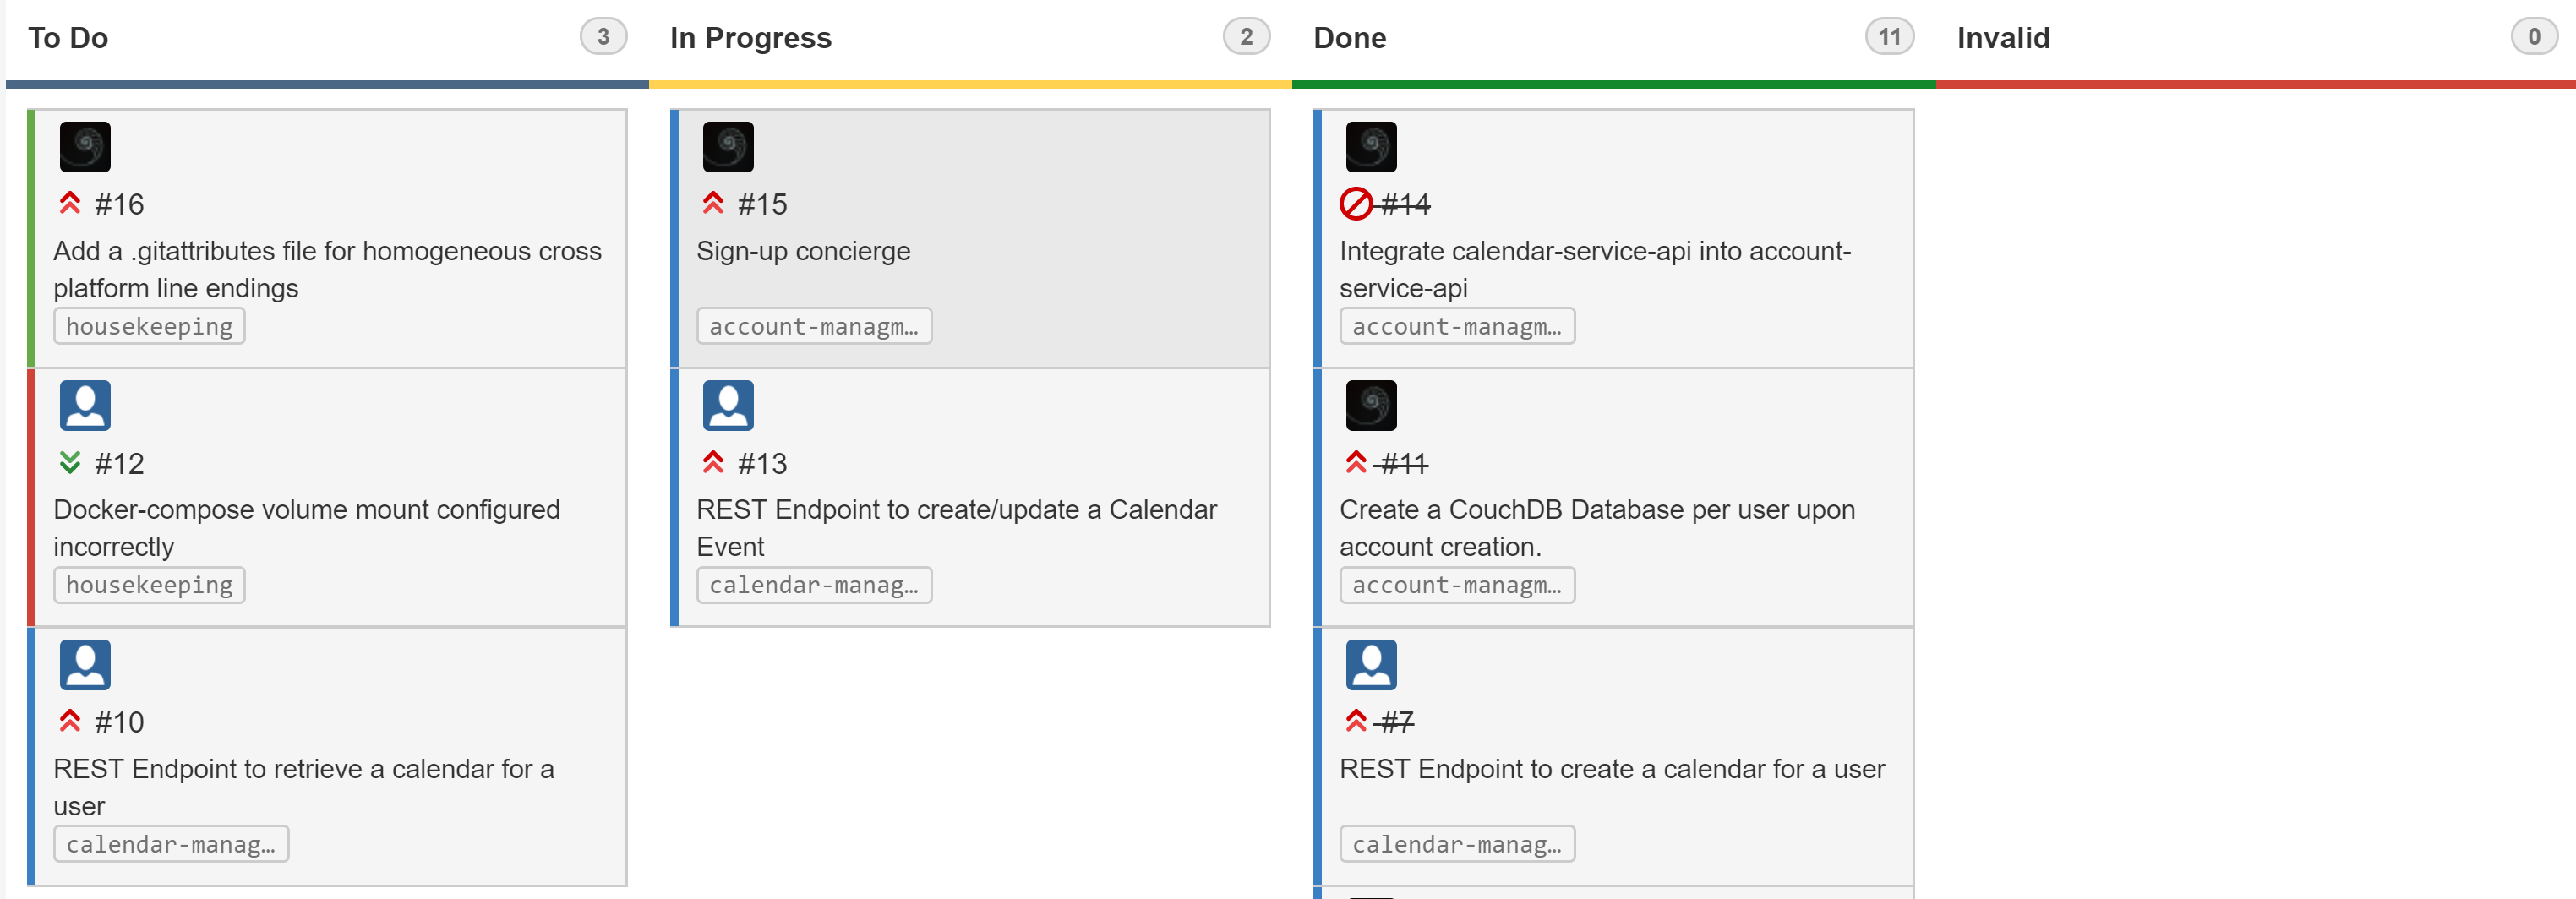
\includegraphics[width=\textwidth]{img/Kanban.PNG}
\caption{Kanban Board}
\label{fig:kanban}
\end{figure}

\paragraph{}In the Figure \ref{fig:kanban} example a couple of tasks have been created, each given their priority as well as the component they relate to and displayed on the board in the To Do state. A developer can come and move a task from the To Do state into the In Progress state to signify that this task is now being worked on. In order to protect the main development / master branch from becoming corrupted by merge conflicts, where numerous developers may be editing the same segment of work, when a task is started a new branch is created off of the development branch\cite{driessen}. See \ref{fig:branches}

\begin{figure}
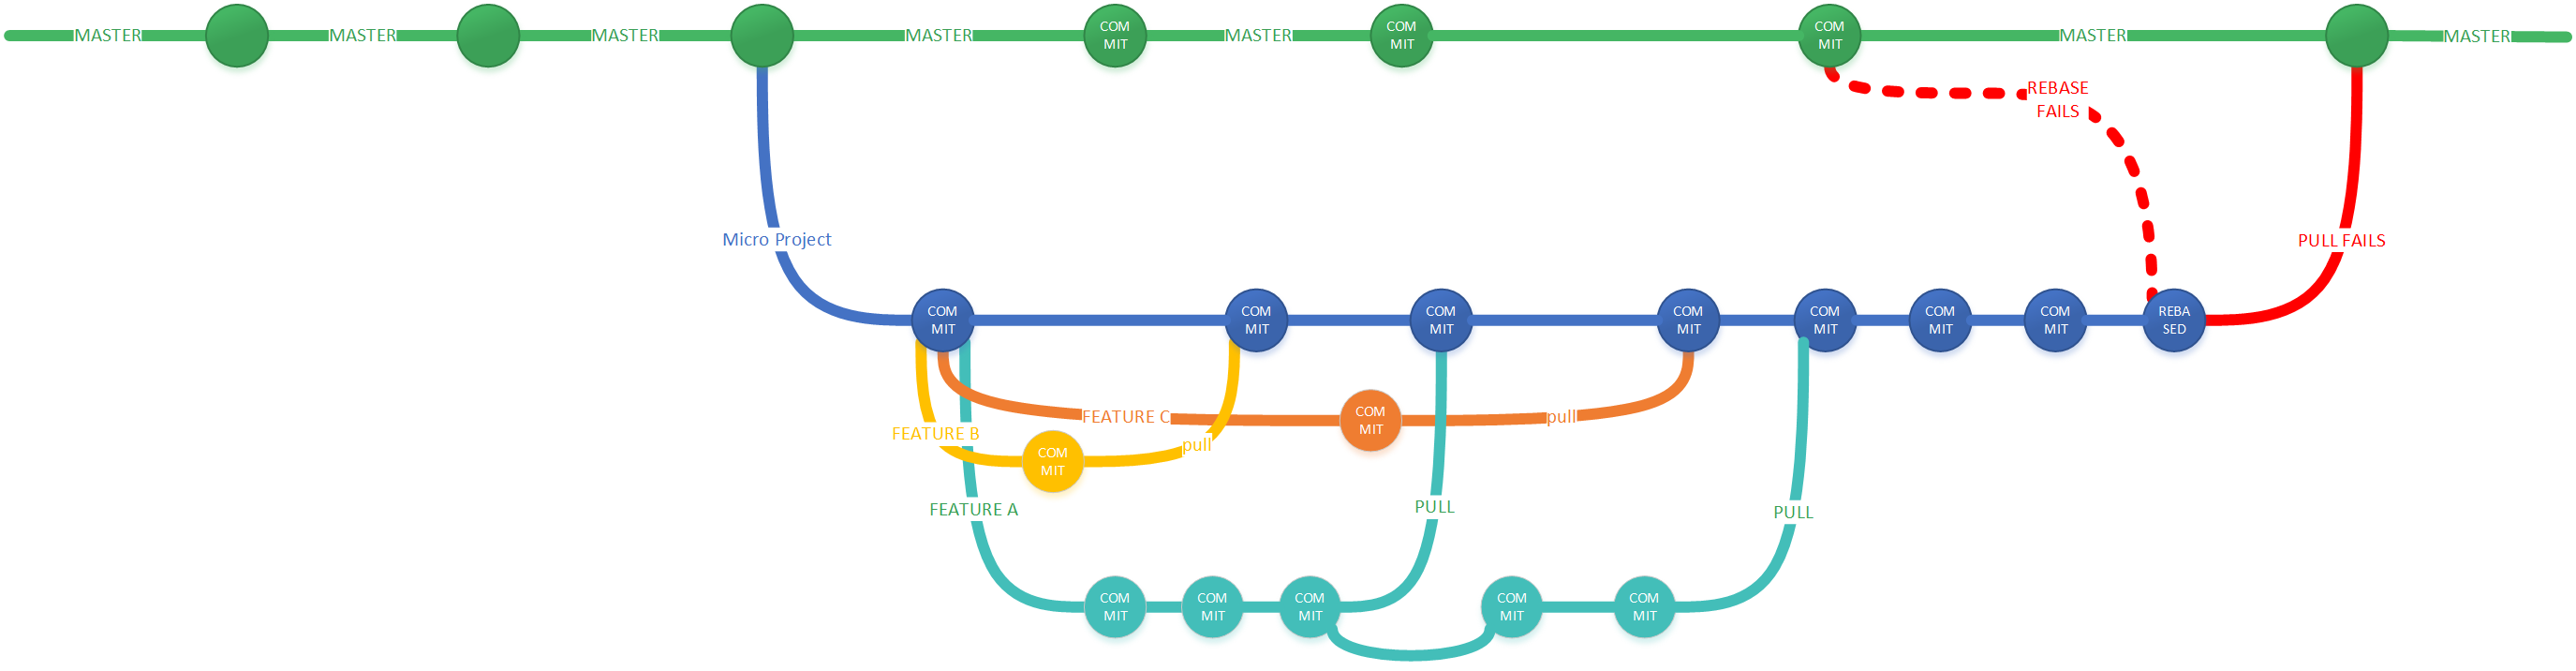
\includegraphics[width=\textwidth]{img/branch.png}
\caption{Git branches}
\label{fig:branches}
\end{figure}

\paragraph{}
Once the task is finished passing all integration and acceptance tests, moved into the DONE state. Before a task can be put into the Done state the developer assigned to the task, must create a Pull Request for the task, which in turn will be reviewed by their colleagues / management to confirm that the task meets the specification of the task, conforms to the quality requirements expected, and works as expected\cite{driessen}.

\section{Slack}

Slack is a team collaboration and services tool used by Software Engineering teams world-wide in the development process of software products. With the use of Slack, team members can stay in touch and comment in numerous different chat rooms for sharing code, reporting bugs and general conversation which may be valuable to product development. The use of Slack throughout the software development life cycle in My Consultancy Services proved to be a beneficial and truly invaluable piece of communication software for working remotely and interacting online. Weekly or fortnightly meetings were held in place between the interns and lead product manager. This helped in providing clarity of arising issues and tutoring of new technologies which were implemented throughout development.